\section{Modeling of W+jets background shape in \texorpdfstring{$m_{jj}$}{dijet invariant mass} }
\label{sec:wjetsShape}
%%%%%%%%%%%%%
%\begin{figure}
%\begin{center}
%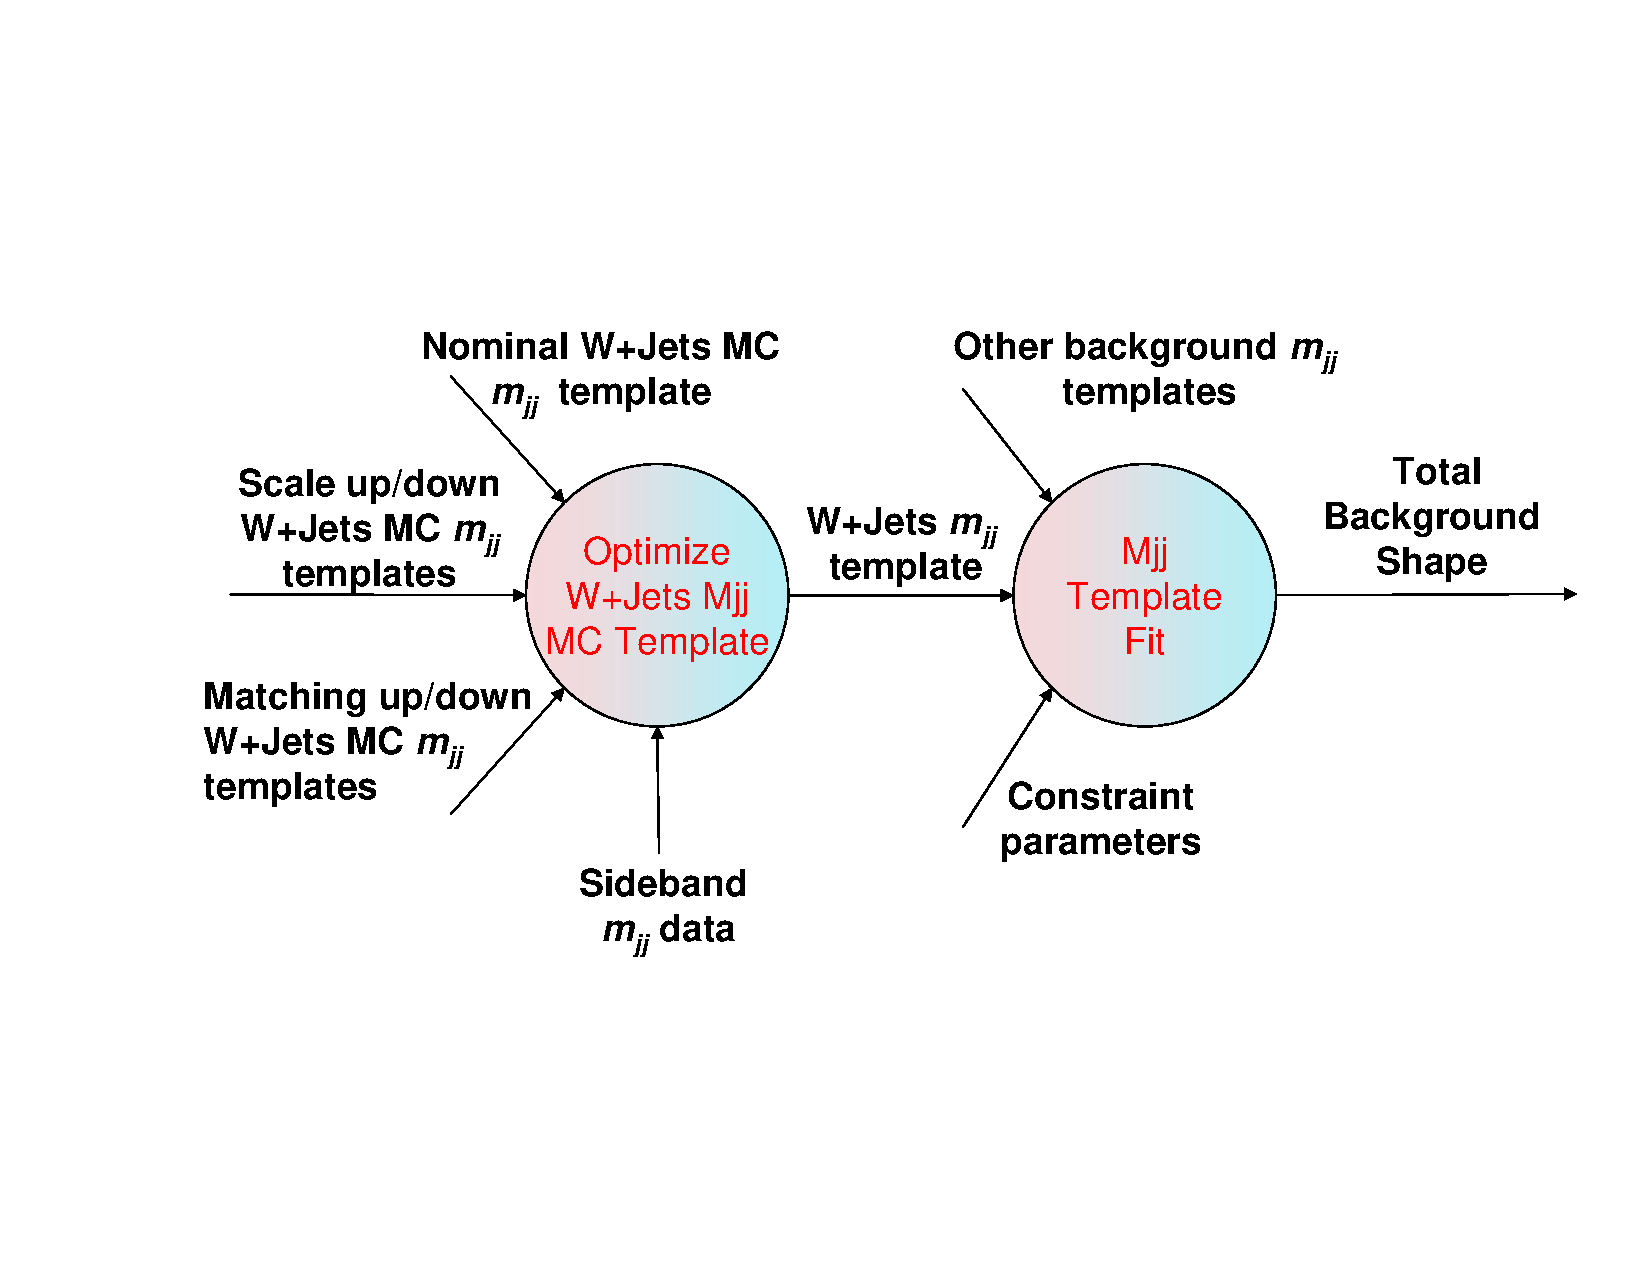
\includegraphics[width=\textwidth,trim=0 150 0 150,clip]{plots/2012_WJetsShape/mjjdfd2body.pdf}
%\end{center} 
%\caption{\label{fig:mjj2body}A depiction of the inputs and work flow of the W+jets template and the final fit.}
%\end{figure} 
%%%%%%%%%%%%%

To determine the expected number of W+jets events in the signal region,
it is necessary to know its shape in the $m_{jj}$ variable.

% In order to get a good description of the W+jets shape in data, the
% simulation needs to describe well both the matrix elements for the
% hard processes, and the subsequent development of the hard partons
% into jets of hadrons.  However, no factorization theorem exists to
% rigorously separate these two components.  A given (n + 1)-jet event
% can be obtained in two ways: from the collinear/soft-radiation
% evolution of an appropriate (n + 1)-parton final state, or from an
% n-parton configuration where hard, large-angle emission during its
% evolution leads to the extra jet.  A factorization scheme defines, on
% an event-by-event basis, which of the two paths should be followed.
% The two relevant parameters defining such a scheme are: the
% factorization/renormalization scale $q^2$ and the matrix element -
% parton shower matching threshold.  Optimized values of these
% parameters should give the best possible approximation to the W+jets
% kinematics for a given fixed-order calculation.  We know that the
% physics has to be independent of the relative contributions of the two
% components.  Therefore, it is important to assess the uncertainty in
% the W+jets shape due to the these unknown parameters.

% %%%%%%%%%%%%%%%
% \begin{figure}
% \begin{center}
% \includegraphics[width=0.6\textwidth]{plots/2012_WJetsShape/Wjets_shapes.pdf}
% \end{center}
% \caption{\label{fig:wjetshapes}The $m_{jj}$ distribution in W+jets events for various
% MC samples.}
% \end{figure}
% %%%%%%%%%%%%%%%


% \par The CMS MadGraph W+jets production uses MLM matching
% \cite{Hoche:2006ph} with $k_T$ jets.  The default matching threshold
% is 10~GeV (i.e., if the parton $p_{T}$ is greater than 10~GeV, then it
% is assumed to have originated from the hard scattering process and
% contributes to the matrix element calculation; if the parton $p_{T}$
% is less than 10~GeV then it is assumed to come from the parton
% shower).  The factorization/renormalization scale $q^2$ corresponds to
% the ``transverse mass'' of the W boson: $\sqrt{M_W^2 + p_{T, W}^2}$.
% 
% To perform studies of the uncertainty due to the choice of
% the $q^2$ and matching scales, alternative MadGraph W+jets samples are
% produced in which the corresponding scales are changed by a factor of 2.
% Thus, we have ``matching-up'', ``matching-down'', ``scale-up'', and
% ``scale-down'' samples, each yielding an $m_{jj}$ distribution, or
% template.  
% Our use of these templates is shown schematically in
% Fig.~\ref{fig:mjj2body} and described below.
% Figure~\ref{fig:wjetshapes} shows representative differences in the MC
% $m_{jj}$ shapes that are availible.

Because of inadequate statistics in the W+jets MC and the overal poor
agreement between W+jets MC and many data distibutions, we employ an
emperical description of the W+jets shape.  This description is a
kinematic turn on and a power law tail:
\begin{equation}
  \mathcal{F}_{W+\text{jets}} = \text{erf}(m_{jj}; m_0, \sigma)\times\left[(m_{jj})^{-\alpha-\beta\ln(m_{jj}/\sqrt{s})}\right]\,,
\end{equation}
where $m_0$ is the value of the turn on and $\sigma$ is the width of
this turn on.  The parameters $m_0$, $\sigma$, $\alpha$ and $\beta$
are determined in the fit to the data after the MVA cut.

This nominal fit shape is not particularly well suited for all of the
mass points.  In the 2-jet channels for masses from 180 GeV and below
we use the MC morphing technique used in the study of the W+2 jets mass spectrum analysis
documented in CMS AN-2011/266, Section 12.  These lower mass points do not suffer from the lack of statistics as they are background
rich, particularly in W+jets background.  We also use the MC morphing technique for 3-jet mass points from 200 GeV 
and below.  We use the following parameterization for 2-jet mass points 190 and 200 GeV.
\begin{equation}
  \mathcal{F}_{W+\text{jets low mass, 2 jets}} = \text{erf}(m_{jj}; m_0, \sigma)\times(m_{jj})^{-\alpha}\times\exp(m_{jj}\tau)\,,
\end{equation}
where the parameters $m_0$, $\sigma$, $\alpha$ and $\tau$ are
determined in the fit.  In the 3-jet channels we use the
parameterization
\begin{equation}
  \mathcal{F}_{W+\text{jets low mass, 3 jets}} = (m_{jj})^{-\alpha-\beta\ln(m_{jj}/\sqrt(s))}\times\exp(m_{jj}\tau)
\end{equation}
for masses 250 and 300 GeV.  These functional line shapes are motivated by the W+jets MC, however their parameters 
are derived strictly from data in the $m_{jj}$ sidebands around the W mass.